\documentclass[tikz,border=4pt]{standalone}
\usepackage{ctex}
\usepackage{amsmath}
\usepackage{pgfplots}
\pgfplotsset{compat=1.18}
\begin{document}
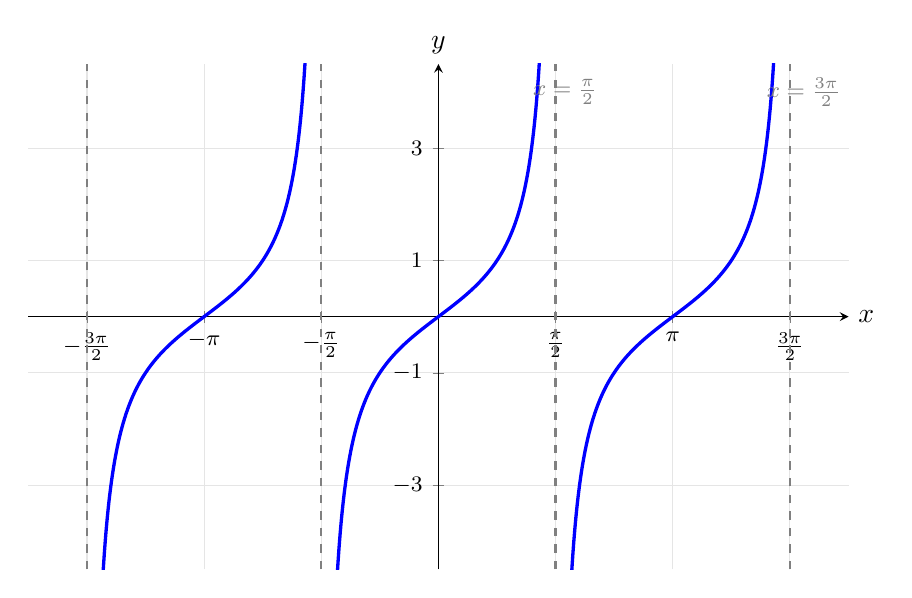
\begin{tikzpicture}
\begin{axis}[
    axis lines=middle,
    xmin=-5.5, xmax=5.5,
    ymin=-4.5, ymax=4.5,
    width=12cm, height=8cm,
    xlabel={$x$}, ylabel={$y$},
    xlabel style={right}, ylabel style={above},
    samples=400,
    grid=both,
    grid style={gray!20},
    xtick={-4.7124,-3.1416,-1.5708,0,1.5708,3.1416,4.7124},
    xticklabels={$-\tfrac{3\pi}{2}$,$-\pi$,$-\tfrac{\pi}{2}$,$0$,$\tfrac{\pi}{2}$,$\pi$,$\tfrac{3\pi}{2}$},
    ytick={-3,-1,1,3},
    tick label style={font=\footnotesize},
    restrict y to domain=-5:5,
]
% tan 主分支
\addplot[blue, very thick, domain=-1.45:1.45] {tan(deg(x))};
\addplot[blue, very thick, domain=1.6924:4.5540] {tan(deg(x))};
\addplot[blue, very thick, domain=-4.5540:-1.6924] {tan(deg(x))};
% 渐近线
\addplot[gray, dashed, thick] coordinates {(1.5708,-4.5) (1.5708,4.5)};
\addplot[gray, dashed, thick] coordinates {(-1.5708,-4.5) (-1.5708,4.5)};
\addplot[gray, dashed, thick] coordinates {(4.7124,-4.5) (4.7124,4.5)};
\addplot[gray, dashed, thick] coordinates {(-4.7124,-4.5) (-4.7124,4.5)};
\node[font=\footnotesize, gray] at (axis cs:1.7,4.0) {$x=\tfrac{\pi}{2}$};
\node[font=\footnotesize, gray] at (axis cs:4.9,4.0) {$x=\tfrac{3\pi}{2}$};
\end{axis}
\end{tikzpicture}
\end{document}
